\section{Experimentation}
\label{sec:experimentation}

To provide some initial experiments, we implemented a model similar to the classic grid world problem. The agent may move north, south, east, and west in a $w$-by-$h$ grid world. The agent moves successfully with a $0.8$ probability, and fails by moving right or left, each with a $0.1$ probability. At the edges, if the agent cannot move, it remains still.

Throughout the area, dead ends are placed (denoted by ``-'') as well as goal states (denoted by ``+''). In the normal MDP version, dead ends have a reward of $-\infty$, and only have a positive weight of $1.0$ on the transition probability for remaining in the dead end. Goal states have a reward of $1.0$, and all other states have a small penalty of $-0.03$.

In our MOMDP with lexicographic reward function model, we separate the dead ends and goal states into two reward functions. The first reward $R_1$ provides a $0.0$ reward for all states, and a $-1.0$ reward for transitioning to a dead end. The second reward $R_2$ yields a $1.0$ for transitioning to a goal state, and a $-0.03$ for all other states.

Figures~\ref{fig:seed_1},~\ref{fig:seed_2}, and~\ref{fig:seed_3} show output from the model in this domain. Interestingly, it appears to work very well at strictly avoiding dead ends, and then optimizing around the remaining action possibilities.
\begin{figure}[h]
    \centering
    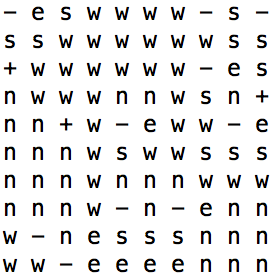
\includegraphics[width=0.4\textwidth,bb=0 0 279 280]{seed_1.png}
    \caption{First example's policy.}
    \label{fig:seed_1}
\end{figure}

\begin{figure}[h]
    \centering
    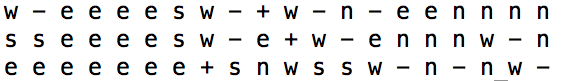
\includegraphics[width=0.4\textwidth,bb=0 0 561 81]{seed_2.png}
    \caption{Second example's policy.}
    \label{fig:seed_2}
\end{figure}

\begin{figure}[h]
    \centering
    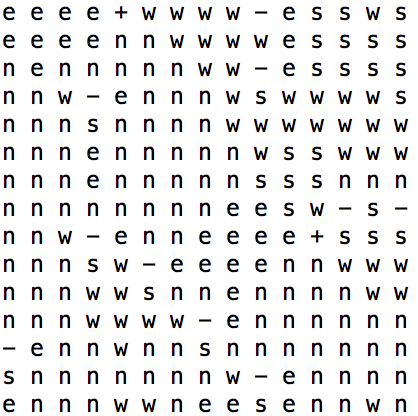
\includegraphics[width=0.4\textwidth,bb=0 0 418 416]{seed_3.png}
    \caption{Third example's policy.}
    \label{fig:seed_3}
\end{figure}

There are additional scenarios for which $\lvmax$ is useful. If there are primary and secondary goals, they can be represented by different rewards, with primary goal states strictly favored over secondary goal states. 
